\chapter{Survey} \label{chap:Survey}

The process of developing hypothesises is an iterative one and, although the first phase of this research resulted in a set of patterns and categories of attribution themes, it is necessary to continue the exploration by validating the findings. Validation in such case, does not relate to the identification of behaviours that cause a dispositional attribution, nor directly to the content of the attribution, but rather to the frequency of certain attributions. Behaviours and biases were collected individually in each interview, and the open-ended questions provided a rich and broad knowledge base, which needed to be further systematized. 

Therefore, a survey in the form of a self-administered questionnaire would be a appropriate method to validate the assumptions from the previous phase. If the possibility arises, even gain more insights. These two generic principles accompany the design process of the questionnaire, which will be described in the next section. The second part of this chapter will be dedicated to the analysis of the questionnaire results, namely in Analysis \ref{Analysis}. This chapter concludes with the Limitations \ref{chapt5:Limitations} that characterize the survey.

Throughout the sections of this chapter the terms \textit{response}, \textit{statement} and \textit{attribution} are often used interchangeably but refer to different things in different contexts. \textit{Response} relates to the answers of the survey, whether predefined or not. \textit{Statement} relates to the formulation of the responses in the closed questions and represents compilations of statements from the interviews. These statements embody \textit{attributions}, which are the core topic under study.

\section{Questionnaire Design Process} \label{questionnaireDesignProcess}

The design of the questionnaire required several steps, starting from setting the objectives, formulating the questions, selecting the right format and distribution to mention a few. These processes unfolded iteratively until the survey reached its final form. This section is divided based on the steps described in \cite{Scheuren2004} and \cite{Fink2003}, in order to explain the realization details in a more orderly manner.

\subsection{Objectives}

In the previous phase, the one of \textit{Interviews}, we received compelling information regarding the most prominent inappropriate behaviours and their accompanying \textit{dispositional} attributions.  Now, we seek to quantify these attributions, and conclude on the most common attributions in general, but also in regards to a specific behaviour.

More specifically, there is one minor and two major objectives that are tackled through the survey. Initially, we aim at gathering insights regarding the intensity of the attributions. Through descriptive statistics, attributions can be analyzed to reach conclusions such as their commonality or frequency.

A follow-up outcome from descriptive statistics is the identification of the behaviours that are more likely to cause a perceiver to make a dispositional attribution. This information will provide more information on the behaviours that concern or irritate the perceivers.

Another important part of the research is to observe whether a correlation between the attribution tendency or levels and leadership traits exists. The latter is important not only to investigate the causes of the attribution error, but also to give meaning to the way project leaders react to certain behaviours. Considering the feedback from the interview design described in \ref{DesignProcess} and prior research conducted in the topic of leadership, it was observed that the attribute of \textit{trust} received considerable attention. \textit{Trust} is one of the hallmarks of the personality trait of \textit{agreeableness} \cite{Kuhnert1987} and \textit{agreeableness} has emerged as the strongest and most consistent predictor of transformational leadership behaviour \cite{Judge2000}.

\subsection{Planning and Development}

When designing a survey, two are the most important aspects that require specific focus: the \textit{questions} and the \textit{responses}. 

Questions in a survey can be closed or open. Since we want to conduct statistical analysis and interpretation of certain biases, the questions require to be closed questions. In closed questions, the answers need to be acquired by the designer. In our case, this process is facilitated by the outcome of the interviews. 

During the design, there were also edge cases that needed to be addressed in order to minimize the researcher's bias. Such cases include interview answers that could not be part of the questionnaire responses, due to the length of each question. Additionally, not every interviewee was faced with every behaviour, and was not able to provide attributions towards each one of them. Moreover, the respondents of the survey might form a situational attribution, which does not correspond with any of the responses, but still represents valuable information. Considering these points, we found it necessary to provide an open question after each closed question. 

The selection of the appropriate questions was also an important step, which drew inspiration from the patterns identified in the interviews. There were a few criteria to be considered: 
\begin{itemize}
    \item The questionnaire needed to have a limited number of questions, otherwise it would become too long and uninteresting to the recipient 
    \item The behaviours that were considered grey areas were the most interesting to study
    \item Completely new, "virtual" behaviours had priority
    \item Behaviours with a larger number of biases, which corresponds to the most mentions by the PLs, also had priority
    \item The behaviours with very few mentions could be excluded
\end{itemize}

Regarding the responses, different options were taken into consideration. First, an alternative-based questionnaire was considered, in which the responder could choose the statement that would best fit their perception. Furthermore, we would equip each question with the possibility to select \textit{other} as an option, and a text field in which more information could be added. Ultimately, it was reasoned that this type of answer would limit the identification of other biases mentioned in the alternatives of the questions. Additionally, the number of participants would remain the same as before, namely ten, and the usage of categorical response choices could result in insufficient data. Comparatively, ordinal responses would produce insights on all the options rather than selecting the most "fitting" alternative out of a few. 

The typical ordinal data collection method is using scales to rate the given statements. In this thesis, we opted for the Likert scale. Since the development of the Likert scale, named after the inventor, Rensis Likert, many researchers have developed instruments to measure particular attributes or traits of individuals or groups \cite{Allen2007}. The instruments usually require respondents to give their level of agreement or disagreement, which can range from 1 to 5, to the statements relating to the attribute being measured. Such a design fits the requirements of this study, and the responses of the questions were evaluated on a five point Likert scale in an order of 1 for Strongly Agree and 5 for Strongly Disagree. 

The process of writing the responses required several iterations and made direct use of the answers PLs gave in the interviews. Some of the answers would be similar, or within an answer, one or more attributions would be identified, which required a careful examination of the answers. The response statements must be easily distinctive, therefore a mix of both combinations and separations of answers resulted in the end-statements.

Other aspects that were considered during the design of survey questions include:
\begin{itemize} 
	 \item Formulating phrases in such a way that the dispositional attribution was clear to identify 
	 \item Provide answers that are not too difficult even for a willing respondent to answer
	 \item The statements should not be repeating themselves or sound too similar
\end{itemize}

The survey was decided to be completed using a digital form, therefore, a web-based platform was investigated. Different platforms for the conduct of the survey were considered, from which, Microsoft Forms was selected, due to its flexibility in the design and the unlimited set of questions offered to TUM students. Most importantly, on this platform the questionnaire could be filled anonymously, which was one of the core requirements of the survey. Anonymity would enable the respondents to freely choose the answer, without fear of being judged and without any external influence.

\subsection{Pretest and final questionnaire}

Before the distribution of the online questionnaire to the participants, undergoing a reviewing phase by an external entity was considered crucial to the identification of weak points. The questionnaire was tested with one of the PLs, who also provided unbiased feedback.

Specific feedback on the questions related to the usage of words that are misspelled or can be difficult to understand by the majority of participants. The feedback also pointed out at questions that could be ambiguous to the respondent. These points were taken into consideration for the final version of the questionnaire.

More general feedback related to the nature of the response statements. One of the suggestions stated the introduction of a "logical excuse option" in the questions, in order to "push out the biases even more". The "logical excuse option" refers to the situational attribution over a behaviour. After thorough consideration, it was concluded that such a change would not add more value to the questionnaire, as the participants would already have two options to their disposal, for the case the dispositional attribution is absent. One instance is the choice the participant to disagree with the statements or answer with "Neutral". Another way is answering the open question provided after each closed questions, which was designed to serve exactly the purpose of accommodating further attributions. Additionally, the introduction of the situational attribution would require further investigations in the previous phase, namely the interviews, as the focus of the questions should have included the situational attribution explicitly for every dispositional attribution. Another risk of introducing such a statement would be influencing the participants towards not admitting to dispositional attribution. This could interfere with the goal of the survey, especially considering that three of the participants showed little to no dispositional attribution tendencies during the interviewing process. 

In the final version of the questionnaire, there is no specific order of the questions regarding the attribution error. The questionnaire starts with the block of closed questions, each equipped with Likert-scale responses. After each closed question, an open one follows. The last question, refers to the identification of \textit{agreeableness} and \textit{trust} levels in the participants, and was ranked as last, to minimize the bias these questions would have on the previous questions. In the creation of these statements, personality tests regarding the Big Five or OCEAN\footnote[1]{https://www.truity.com/book/big-five-personality-model} traits were considered, more specifically the ones on agreeableness and trust\footnote[2]{https://www.truity.com/test/how-agreeable-are-you}. 

Additionally, the closed question were set as required, so that every participant would input the data. The open ones were considered optional. 

After approval of the final set of questions, the questionnaire was distributed electronically through messaging applications such as RocketChat and Slack, which were used to contact the participants in the first phase of this study as well.

The  finalized version of the survey can be found in~\autoref{tab:table6}.

\section{Analysis} \label{Analysis}

The analysis methods selected were highly dependent on the type of data and the context we were working with. In our case study, we did not aim at making assumptions for the whole population, therefore, we were dealing with non-parametric data. Additionally, the type of responses from the survey closed questions qualify as \textit{ordinal data}, considering the ranking that is made between "Strongly Disagree" (marked by the value of 1) and "Strongly Agree" (marked by the value of 5). As a general rule, mean and standard deviation are invalid parameters for descriptive statistics whenever data are on ordinal scales, as are any parametric analyses based on the normal distribution \cite{Allen2007}. Non-parametric procedures (based on the rank, median or range) are appropriate for analyzing these data, as are distribution free methods such as tabulations, frequencies, contingency tables and chi-squared statistics \cite{Sullivan2013}. 

There are though exceptions which tolerate the use of mean for statistical description. Such a case is when researchers are attempting to measure less concrete concepts, such as motivation,  satisfaction, and confidence, where a single survey item is unlikely to be capable of fully
capturing the concept being assessed \cite{Rickards2012}. Another prerequisite of using the mean to describe the central tendency, is that the items of the survey must measure the same underlying variable \cite{Sullivan2013}. In our case, this variable is the tendency each respondent has to form a specific attribution. Furthermore, we assume that the psychological difference between "Strongly Agree" and "Agree" is the same as "Agree" and "Neutral".

After an initial analysis of median, mean and range, it was identified that the mean provided more context to the data, and a more accurate dissection of the levels of attribution. Consequently, we made use of the mean to derive a first interpretation of the data. The following formula \eqref{Interpretation} describes the initial point of interpretation, where $\bar{x}$ symbolizes the mean of the data set related to a questionnaire response:

\begin{equation} \label{Interpretation}
Interpretation =
    \begin{cases}
      \textit{Very strong attribution,} & \text{if } 4.5 \leq \bar{x} \leq 5.0 \\
      \textit{Strong attribution,} & \text{if } 3.5 \leq \bar{x} < 4.5 \\
      \textit{Mild attribution,} & \text{if } 3.0 \leq \bar{x} < 3.5 \\
      \textit{Not an indicator of strong attribution,} & \text{otherwise}
    \end{cases}       
\end{equation}

The scale we choose for the interpretation corresponds to the tendency for an attribution to be made. After this initial categorization, the medians, the ranges and often the frequencies aid with the analysis of the nuanced response data, especially the ones lying at the edges of the cases. There are often instances, in which attributions have been made, but the mean result does not accurately reflect the right intensity. Therefore, the final interpretation considers the above mentioned techniques of data description too. All relative frequencies of the questionnaire responses can be found in ~\autoref{tab:AttributionResponsesFrequencies}.

Part of this study is also finding a correlation between agreeableness and dispositional attribution tendencies. In order to achieve this, before statistically analysing the data, the ratings given as responses were summed to derive an overall score, once for the \textit{agreeableness} score and once for \textit{attribution bias tendencies}. This resulted in the creation of \textit{interval data}, which could then be analyzed through new methods, targeted at this kind of data. Such a method is Pearson's correlation coeffiecient.

\subsection{Attribution tendencies}

The following~\autoref{QuestionnaireResponsesInterpretation} displays the results of the analysis on attributions. The \textit{Question} and \textit{Attribution} columns present codes for the questionnaire closed questions and their respective responses/statements/attributions. The original questionnaire with the codes can be found in~\autoref{tab:table6}. The next three columns represent the statistical methods we use to describe the data, namely the \textit{Median}, \textit{Mean} and \textit{Range}. The last column represents the final interpretation of the data on one statement, following the methodology described in the introduction of this section. The interpretation often provide more explanations, in order to adequately describe the phenomenon of attribution in this survey.

 
\begin{longtable}{  c | c  | c | c | c |  p{0.35\textwidth} }
\caption[Questionnaire responses' interpretation]{Questionnaire responses' interpretation}\\
% \centering
    %\begin{tabular}{clcccccccccc}
    \hline
       \textbf{Question} & \textbf{Attribution} & \textbf{Median} & \textbf{Mean} & \textbf{Range} & \textbf{Interpretation}  \\
        \hline
        Q1
        & \textbf{A1.1}
                     & 4 & 4.3 & 2  &  Strong to very strong attribution, considering only one neutral answer and multiple strongly agree  \\ 
        & A1.2
                       & 4 & 3.78 & 3 &  Strong attribution   \\
        & A1.3  &  4 & 4.1 & 3  &  Strong attribution  \\
        & A1.4   & 4 & 4 & 3  &  Strong attribution  \\
        \hline
        Q2
        & A2.1
                    & 3  & 2.67  &  3 & Not an indicator of a strong attribution \\
        & A2.2
                       & 3 & 2.78 & 2 & Not an indicator of a strong attribution  \\
        &\textbf{A2.3}
                      & 4 & 4.11  & 2 & Strong attribution, no person disagrees \\
        & A2.4
        				& 3  & 2.8  & 3 & Not an indicator of a strong attribution \\
        & A2.4
                      & 3 & 2.9  & 3 & Not an indicator of a strong attribution  \\
       \hline
        Q3
        & \textbf{A3.1}
                    & 5 & 4.6  & 1 & Very strong attribution \\
        & A3.2
                       &  4 & 3.8 & 1 & Strong Attribution \\
        & A3.3
                      & 3 & 3.1  & 2 & Mild attribution  \\
        & A3.4
        				& 3 & 3.4 & 3 & Mild to strong attribution, considering the large range and a higher frequency of total agreement responses \\
       \hline
        Q4
        & A4.1
                    & 3  & 3.2  &  2 & Mild attribution  \\
        & \textbf{A4.2}
                       & 4 & 4.3 & 2 & Strong attribution \\
        & A4.3
                      & 4  & 3.9  &  2 & Strong attribution  \\
        \hline
        Q5 
        & \textbf{A5.1}
                    & 4 & 3.9  & 3 & Strong attribution  \\
        & A5.2
                       & 3 & 3 & 3 & Mild to no attribution, considering Strongly Disagree  \\
        & A5.3
                      & 2 & 2.3  & 1 & No attribution  \\
        & A5.4
        				& 3 & 3 & 3 & Mild attribution \\
        \hline
        Q6
        & \textbf{A6.1}
                    & 4  & 4  &  0 & Strong Attribution   \\
        & A6.2
                       & 3 & 3.1 & 3 & Mild attribution  \\
        & A6.3
                      & 3 & 3  & 3 & Mild attribution  \\
        & A6.4
        				& 4 & 3.6 & 1 & Strong attribution \\
        \hline
        Q7
        & \textbf{A7.1}
                    & 4 & 3.2  & 3 & Mild attribution \\
        & A7.2
                       & 3  & 2.8  & 3 & Not an indicator of strong attribution  \\
        & A7.3
                      & 3 &  3.1 & 2 & Mild attribution  \\
       \hline
        Q8
        & A8.1
                    & 4 & 4  & 2 & Strong attribution   \\
        & A8.2
                       & 5 & 4.6 & 1 & Very strong attribution  \\
        & \textbf{A8.3}
                      & 5 & 4.7 & 1 & Very strong attribution \\
        \hline
        Q9
        & A9.1
                    & 3 & 2.7  & 3 & Not an indicator of strong attribution  \\
        & \textbf{A9.2}
                       & 3 & 2.9  & 4 & Very weak indicator, taking in consideration the large range \\
        \hline
        Q10
        & A10.1
                    & 2 & 2.6  & 2 &  Not an indicator of strong attribution   \\
        & A10.2
                       & 3  & 2.6 & 3 & Not an indicator of strong attribution  \\
        & \textbf{A10.3}
                      & 3 & 2.9  & 4 & Very weak indicator, taking in consideration the large range \\
        \hline
        Q11
        & A11.1
                    & 3 & 3  & 2 & Mild attribution   \\
        & \textbf{A11.2}
                       & 3  & 3,1  & 2 & Mild attribution \\
        & A11.3
                      & 3 & 2.9  & 2 & Not an indicator of strong attribution  \\
        \hline
        Q12
        & A12.1
                    & 4 & 3.6  & 3 & Strong attribution   \\
        & \textbf{A12.2}
                       & 5 & 4.6 & 1 & Very strong attribution \\
        & A12.3
                      & 3 & 2.4  & 3 & Not an indicator of strong attribution  \\
       \hline
        Q13
        & A13.1
                    & 4 & 3.7  & 3 & Strong attribution \\
        & A13.2
                       & 3 & 3 & 2 & Mild attribution \\
        & \textbf{A13.3}
                      & 4 & 3.9  & 2 & Strong attribution   \\
        \hline
        Q14
        & A14.1
                    & 4 & 3.8  & 3 & Strong attribution \\
        & \textbf{A14.2}
                       & 4 & 4 & 3 & Strong attribution \\
        \bottomrule
   % \end{tabular}
   \label{QuestionnaireResponsesInterpretation}
\end{longtable}

From the analysis of the questionnaire data, the results can be summarized as follows:

\begin{itemize}
\item 4 responses very strongly indicate dispositional attribution from the perceiver,
\item one in-between very strong and strong,
\item 15 statements with strong attribution,
\item one statement of mild to strong attribution,
\item 9 statements have been mildly or moderately indicate attribution,
\item 3 statements weakly indicate attribution,
\item 9 statements do not indicate a strong attribution,
\item 1 statements not presenting any attribution as all.
\end{itemize} 

The strongest attribution per question are marked in bold. The four statements with the highest tendency for attribution present no particular commonalities. They individually refer to a person being impolite, immature, disinterested and unapproachable. However, these attributions \textit{can} be clustered together to form personas, as it will be seen in \autoref{Personas}.

\subsection{Attribution-forming Behaviours}

In this section we want to present the behaviours with the highest frequencies of "Agree" responses. More colloquially, we aim at answering the following question: \textit{Which are the behaviours that are more likely to push people towards forming attributions?}

Figure \ref{fig:AgreeablenessFrequencies} depicts the data for the "Agree" and "Strongly Agree" relative frequencies in each of the closed questions of the questionnaire. A third bar displays the total sum of the frequencies. The questions are also sorted by the final outcome, in order to improve the readability of the results.

The behaviours which received the highest attribution rate are Q8, Q14 and Q1. They relate to intense interaction with mobile phones, engaging in physical movements while being in the meeting and joining from their mobile phones, respectively. A common theme which characterizes these behaviours is \textit{distraction}. The biggest distractions PLs mention are screens, whether in a monitor, smartphone, or smart watch. Situational attributions also get mentioned, such as the meeting being boring (presented in Q8) or generally irrelevant (according to a respondent in Q1).

A temporary, physical detachment from the proximity of their typical devices (as viewed in Q14 and Q4, but even Q1), drive the participants to strongly agree to the dispositional attributions presented to them. The respondents perceive the distance to not only be physical, but also mental.

The behaviours that rank the lowest are related to the appearance of the participants. When the face is not entirely visible as in Q10, respondents mention the change of natural light as a factor, or attribute the dark atmosphere to the "nerdness" of a person. In regards to backgrounds, considering that the participants of the iPraktikum are students, a certain level of disorderliness is generally tolerated. The open question responses make a difference between formal and informal meetings, and one response suggests to even appreciate this opportunity to learn more about the participants' personality. In regards to Q11, internet issues are also taken in consideration when forming attributions, but again, when the PLs sense a lack of focus, a tendency to form a dispositional attribution persists.


\subsection{Analyzing the correlation between agreeableness and the tendency for attribution}

The third RQ in this thesis aims at understanding more about the behaviours of the perceivers too, in our case the PLs. Considering the research methods undertaken in this study, we dedicated part of the survey to answer this question as well. The last question of the survey presents the respondents with statements concerning their personality and reactions towards the team members.

As described at the objectives of the survey, leadership studies have been leaning towards the cognitive approaches to information processing and decision making processes \cite{Dinh2014}. These even form the branch of \textit{information processing theories} within leadership theories. Another popular branch of leadership theories looks at individual differences in leaders and investigates specific traits or abilities that contribute to leadership effectiveness. 

In the survey we look specifically at the subject of \textit{Agreeableness} and \textit{Trust}. The statements are built in such a way, that can be directly associated with agreeableness attributes of the responder. The answers to these statements can be found in~\autoref{tab:DispostionQuestionFrequencies}.

\begin{longtable}{  p{0.3\textwidth}   p{0.12\textwidth}  p{0.1\textwidth}  p{0.1\textwidth}  p{0.1\textwidth}  p{0.1\textwidth} }
 \caption[Disposition Question Frequencies]{Frequencies of disposition questions} \\
	\bottomrule
    Statement  & Strongly Disagree & Disagree & Neutral & Agree & Strongly Agree \\
	\bottomrule
    I trust other people almost immediately & 0\% & 22.2\%  & 44.4\%  &   22.2\%  & 11.1\%
   \\
   It's difficult for me to trust other people actually  & 22.2\% & 44.4 \% & 22.2\% & 11.1\% & 0\%
     \\
     I usually get concerned about the well-being of this person and instruct the coach to look into that  & 0\% & 22.2\% & 33.3\% & 44.4\% &  0\% 
    \\
      It is not my responsibility to make others feel better or look after everyone & 0\% & 66.67\% & 22.2\% &  11.1\% & 0\%
      \\
      I am quite sharp-tongued when I get back at others  & 0\% & 66.67\% & 22.2\% & 11.1\% & 0\%
      \\
       I usually try not to contradict others  & 33.3\% & 33.3\% & 22.2\% &  11.1\% & 0\%
     \\ 
    I state my opinion several times since I know which is the right thing to do  &  11.1\% & 11.1\%  & 44.4\%  &   33.3\%  & 0\%  \\
    \bottomrule 
    \label{tab:DispostionQuestionFrequencies}  
\end{longtable}

As observed from the results, the respondents perceive themselves considerably trusting towards others. 66.6\% of the respondents have no difficulty trusting other people, but only 33.3\% agree to trusting others almost immediately, which is indeed a more exaggerated statement. The third and the fourth statement responses also point towards a disposition to provide a comfortable environment for the participants. 66.67\% see a responsibility to improve this environment, but less people get concerned about the well-being of the team (44.4\%). The last three statements describe the leader's need to dominate within the team. Interestingly, 66.6\% of the participants have no problem contradicting others.

To calculate the correlation between the tendency to form attributions and the disposition of agreeableness, every participant's answers were summed to achieve one total score for each of these variables. These scores served as the input for the calculation of \textit{Pearson's correlation coefficient}, which takes the values from -1 to 1. 

In order to generate as many insights as possible and to look closer into the topic of \textit{trust}, multiple calculations were performed. Initially, all questions and statements were subject to this computation. In the next rounds, the questions with the highest frequency of agree answers were under study, starting from the thresholds of 50\% and continuing to 75\%. Another interesting set of attributions were the ones which received 50\% or more "Agree"-s, regardless of the questions they were part of. The last row of the table, represent this group of data.

The statistics we derive are shown in third and fourth columns of the table. r(7) denotes the result of \textit{Pearson's r} or \textit{Pearson's correlation coefficient}, with 7 being the degrees of freedom (calculated as N - 2). The presentation form of the coefficient follows the APA Style Guidelines \footnote{https://www.socscistatistics.com/tutorials/correlation/default.aspx}. The last column gives an interpretation of the resulted coefficient. Meanwhile, the second column indicates the  agree frequency of the question with the lowest value in the group. This value is missing for the last row, as no specific questions are being considered.

\begin{longtable}{  p{0.2\textwidth}  p{0.12\textwidth}  p{0.1\textwidth}   p{0.1\textwidth}  p{0.3\textwidth} }
\caption[Pearson's coefficient results]{Pearson's coefficient results} \\
  \hline
  \hline
    Subjects under consideration & Lowest frequency  & r(7)  & r(7) - only trust & Meaning \\
    \hline
    \hline
    All Questions and Statements & 22.22\% &  -.01 & -.11 & Although technically a negative correlation, the relationship between the variables is only weak   \\
    Q12, Q6, Q13, Q3, Q4, Q1, Q14, Q8 & 55.56\% & -.20 & -.23 & Although technically a negative correlation, the relationship between the variables is only weak  \\
    Q1, Q14, Q8 & 77.78\% & -.24 &  -.11 & Although technically a negative correlation, the relationship between your variables is the weak \\
    Statements with over 50\% agree responses &  & -.27 & -.25 & Although technically a negative correlation, the relationship between the variables is only weak \\
    \bottomrule
    \label{tab:PearsonResults}  
\end{longtable}

As denoted in the fourth column of the table, the meaning of the coeffiecient is the same in all cases. Nonetheless, there are tendencies and variations to be further examined in each iteration. 

Generally, there is a weak negative correlation between the attribution tendency and agreeableness or trust in a person. We observe that, as the set of statements is confined to the questions mostly attributed, the correlation slightly increases. The case in which the correlation is stronger, is the one between the statements with the higher agreement rate and agreeableness. 

Trust alone appears to not yield more meaningful results than the total agreeableness score. Therefore, between agreeableness and trust, agreeableness would potentially be a more significant indicator for a low attribution-making tendency.

The more remarkable difference between agreeableness and trust is in the third case, in which only three questions are taken into consideration. This phenomenon happens due to the covariance being lower between attribution tendency and trust in this specific instance.

%http://wjh12.harvard.edu/~dtg/Gilbert%20&%20Malone%20%28CORRESPONDENCE%20BIAS%29.pdf paper on the causes of cerrespondence bias

\section{Limitations} \label{chapt5:Limitations}

Considering the relatively small number of respondents (9 out of 10 responses, 90\% response rate), and the format of the survey, we were limited in the methods we could use for the analysis of data. Furthermore, the identification of correlation increases in reliability the more data is available, and therefore, the results can potentially vary with a larger data set.

The survey provides a high level of reliability due to being written in simple language and following the feedback given after the first test of the survey. Hence, we assume that the content of the survey is understood and interpreted similarly by the different participants of the survey. 

Recalling the small sample under study, external validity is a critical point. Moreover, this case study takes place in a university context, where the majority of the participants in the teams are students in their early adulthood.

The survey is the second part of this research and is built upon the data retrieved from the interviews. Therefore, we consider this phase to serve as a triangulation of the research conducted previously. In principle, it is almost the same data under study in both processes, although the objectives differ. From all the statements representing attributions, only one attribution received no "Agree"-s (out of 46). This serves in itself as an indicator of a high validity.

As the interviewees were asked to evaluate different behaviours in their meetings, four of the interviewees would often admit to exhibiting certain behaviours, and therefore tolerate the same behaviours in others. Considering the survey questions to be more specific and in some cases, more extreme, we assume that this category of respondents have contributed more significantly in the identification of attribution tendency.

Regarding the design of the survey, construct validity is established as the objectives of the survey are addressed. The two major objectives especially, are easily distinguishable in the survey form. Eventually, we were able to deliver an evaluation of the biases PLs form in regards to the disposition of the participants. Moreover, we were able to learn more about the PLs themselves, their agreeableness and ways of interacting.



%Extreme cases did not occur in their meetings. Such behaviours include being distracted in the meetings, reading emails, writing emails, coming late or having to leave early, to mention a few. The more typical atribution error occured for being late at meetings.

\usetikzlibrary{patterns}
\pagebreak
\begin{figure}
\centering
\caption{Histogram of questions' "Agree" and "Strongly agree" relative frequency}
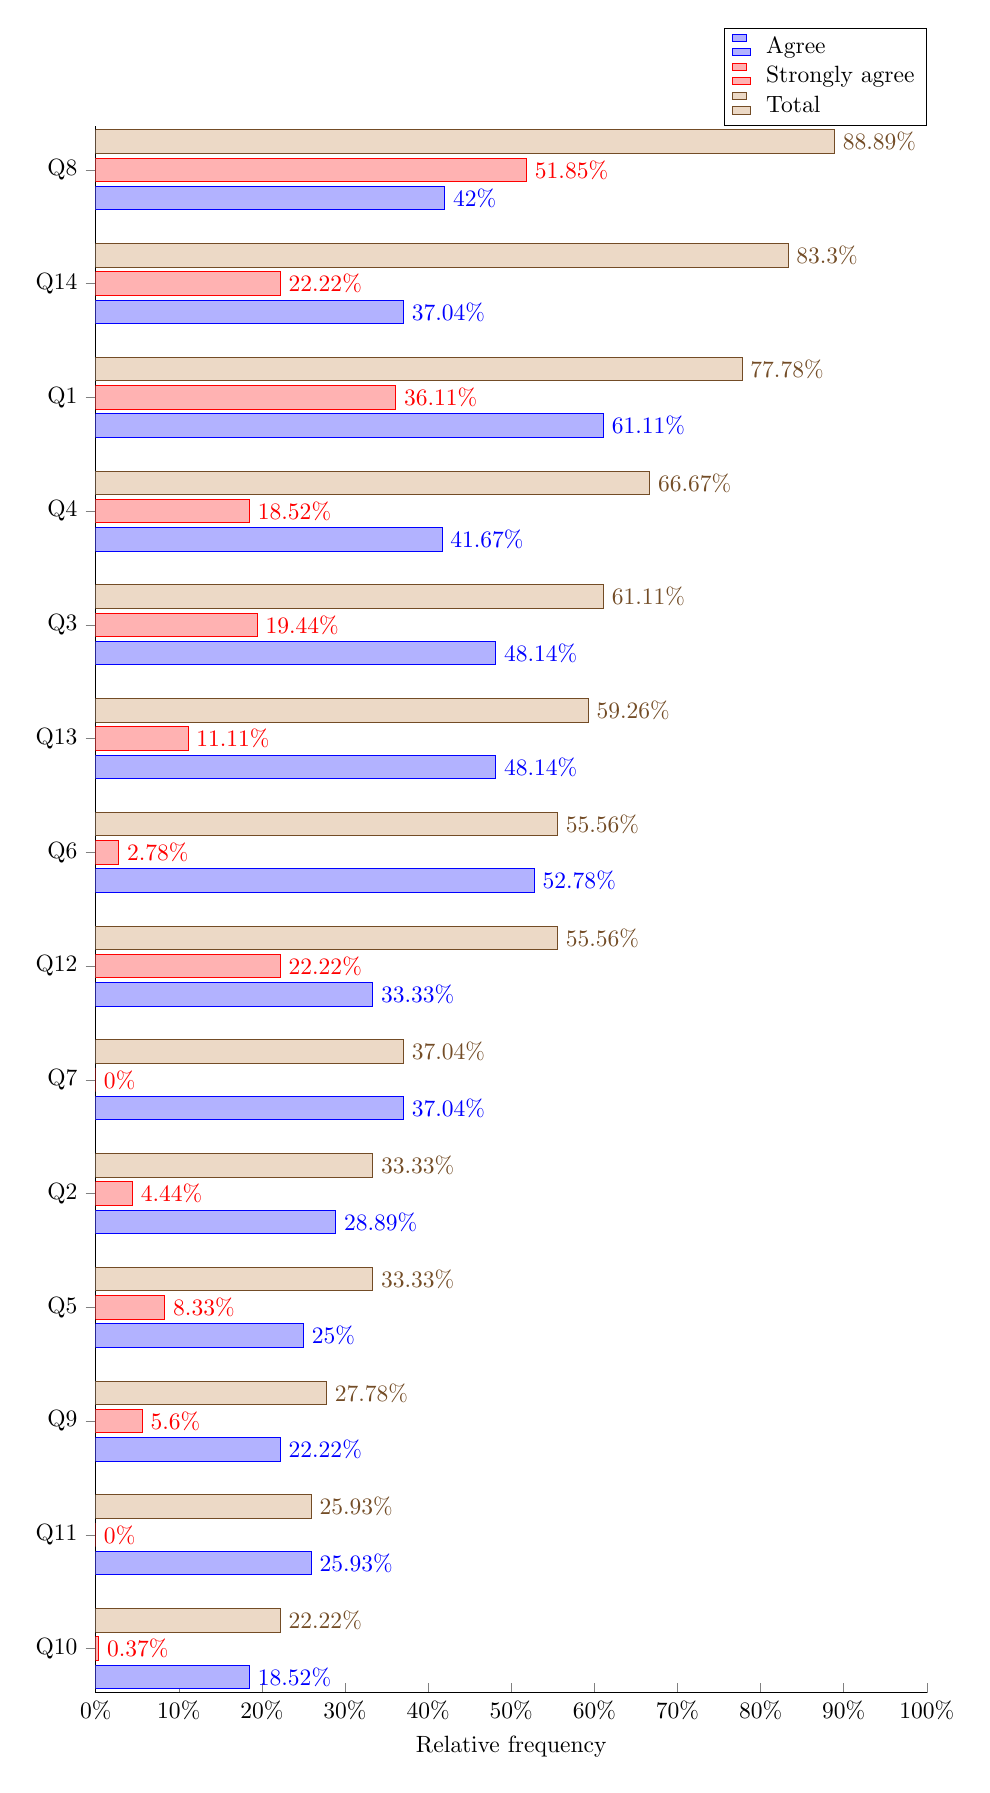
\begin{tikzpicture}[scale=0.85]
\begin{axis}
[
	enlarge y limits=0.03,
    axis lines*=left,
    xbar,
    width=14cm,
    height=25cm,
    xlabel={Relative frequency},
    symbolic y coords={Q10, Q11, Q9, Q5, Q2, Q7, Q12, Q6, Q13, Q3, Q4, Q1, Q14, Q8},
    ytick=data,
    xmin=0,
    xmax=1.0, 
    xticklabel={\pgfmathparse{\tick*100}\pgfmathprintnumber{\pgfmathresult}\%},
    point meta={x*100},
    nodes near coords={\pgfmathprintnumber\pgfplotspointmeta\%},
    nodes near coords align={horizontal},
    legend cell align=left,
        legend style={
                at={(1,1)},
                anchor=south east,
                column sep=1ex
        }
    ]
  \addplot
coordinates
     {(0.1852,Q10)  (0.2593,Q11) (0.2222,Q9) (0.25,Q5) (0.2889,Q2) (0.3704,Q7) (0.3333,Q12) (0.5278,Q6) (0.4814,Q13) (0.4814,Q3) (0.4167,Q4) (0.6111,Q1) (0.3704,Q14) (0.42,Q8)};
  \addplot
coordinates
     {(0.0037,Q10)  (0.0,Q11) (0.056,Q9) (0.0833,Q5) (0.0444,Q2) (0.0,Q7) (0.2222,Q12) (0.0278,Q6) (0.1111,Q13) (0.1944,Q3) (0.1852,Q4) (0.3611,Q1) (0.2222,Q14) (0.5185,Q8)};
      \addplot 
coordinates
     {(0.2222,Q10)  (0.2593,Q11) (0.2778,Q9) (0.3333,Q5) (0.3333,Q2) (0.3704,Q7) (0.5556,Q12) (0.5556,Q6) (0.5926,Q13) (0.6111,Q3) (0.6667,Q4) (0.7778,Q1) (0.833,Q14) (0.8889,Q8)};
     \legend{Agree,Strongly agree, Total}
\end{axis}
\end{tikzpicture}
\label{fig:AgreeablenessFrequencies}
\end{figure}
\pagestyle{empty}